\begin{figure}[t!]
\centering
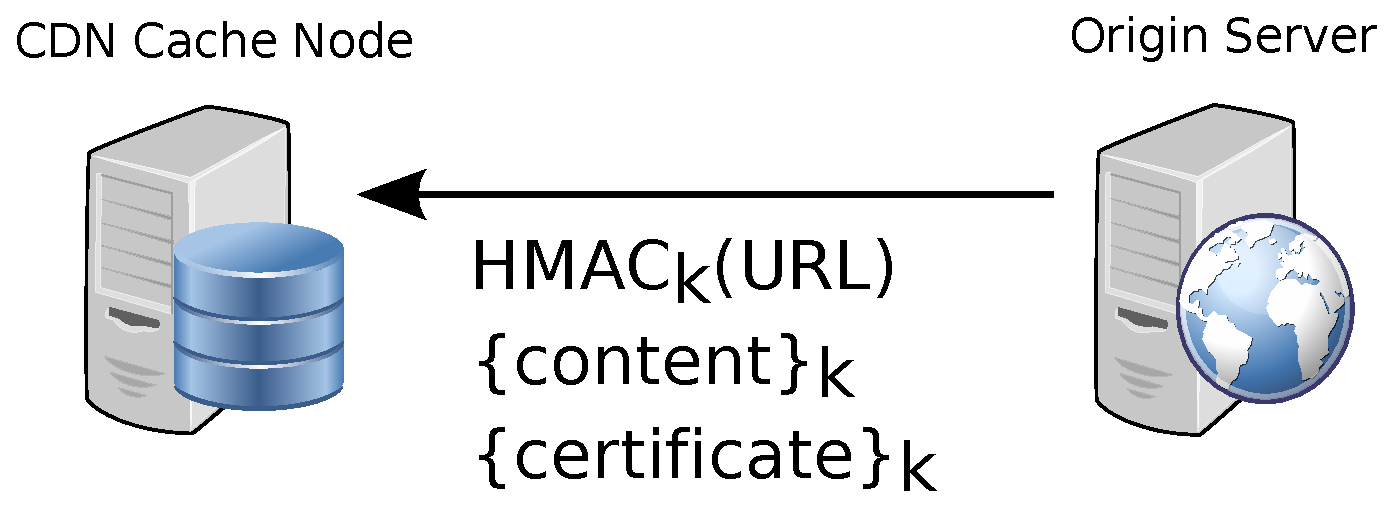
\includegraphics[width=.3\textwidth]{publishing_content_new2}
\caption{Publishing content in \system{}.  $k$ is shared between the 
origin server and the corresponding exit proxy; the CDN has no knowledge of $k$.}
\label{fig:publishing}
\end{figure}

\section{\system{} Protocol}
\label{sec:protocol}
Based on the design decisions discussed in the previous section, we specify the 
steps taken to publish and retrieve content in \system{}. \annie{The \system{} protocol works 
on both plaintext and encrypted requests (HTTP and HTTPS requests).}

\subsection{Publishing Content}
\label{sec:publish_protocol}
To publish content such that the CDN never sees it, the publisher 
must first obfuscate her content, as described in Section \ref{sec:design}. 
Figure \ref{fig:publishing} shows the steps taken to publish content. The most important step in content publishing is obfuscating the data.  We assume that the origin server already has a public and private key pair, as well as a certificate.  To obfuscate the data the origin server will need to generate a shared key $k$. 

Once the key is established, the origin server must first pad the content to the same size for some 
range of original content sizes (i.e., if content is between length x and y, then pad it to length 
z).  The range of content sizes should be small, introducing negligible padding
overhead, but
reduces the probability of identifying the content based on the content length.  This content padding 
is done to hide the original content's length, as it may be identifiable simply by its length.  After 
content is padded, then the content is divided into fixed size blocks and padded to 
some standard length.  Then each block is encrypted using the shared key $k$, 
resulting in a set of encrypted blocks. Because the CDN does not have access to the shared key, 
it cannot see what content it is caching.  

Once the content is obfuscated, the origin server must also obfuscate the content's identifier.  To do so, 
it computes the HMAC of the URL using the shared key $k$.
Once the identifier and the content are obfuscated with $k$, they can be pushed to the CDN, or optionally to multiple 
CDNs.  Recently, services have cropped up to allow and help facilitate the use of multiple CDNs for the same content; an 
origin server could use multiple CDNs' services.  This mechanism could be used in \system{} to increase reliability, 
performance, and availability; an origin server can use a service, such as Cedexis~\cite{cedexis}, to load balance between 
CDNs.  We discuss the use of multiple CDNs more in Section \ref{sec:partial} on \system{} in 
partial deployment.

Because the exit proxies use consistent hashing to divide keys among proxies while
balancing load, the origin server
determines which exit proxy is correct (based on the consistent hashing circle).  The origin server then encrypts the 
shared key $k$ with the correct exit proxy's public key $PK_{exit}$.  
Figure \ref{fig:keys} shows the steps for retrieveing a shared key.  First, the
exit proxy sends a DNS request to the origin server's authoritative DNS server, including its self-certifying
identifier and its public key (these are both included in the {\tt Additional Info} section of the DNS message).  The origin server hashes the exit 
proxy's public key and verifies it against its self-certifying identifier; this acts as a proof of the 
exit proxy's position in the consistent hashing circle.  If the origin is able to certify the exit proxy, then it will send the DNS response with 
\{$k$\}$_{PK_{proxy}}$ in the SRV record. The exit proxy will receive the encrypted shared key, which it can decrypt with it's private key.

\begin{figure}[t]
\centering
\includegraphics[width=.45\textwidth]{key_lookup}
\caption{How an origin server certifies an exit proxy and distributes its shared
key to an exit proxy.  In step~(1), 
the exit proxy sends his self-certifying ID in the {\it Additional} section of the DNS message.  }
\label{fig:keys}
\end{figure}

\textbf{Updating Content.}
For an origin server to update content, it must follow similar steps as described
in publishing content.  
Once it has updated the content on the origin server, it must obfuscate it using
the same steps: 1) pad the 
original content length, 2) divide the content into fixed size blocks, and 3) encrypt the content blocks 
with the shared key $k$.  Because it is updating the content (as opposed to creating
new content), the 
obfuscated identifier will remain the same.  The origin server signs the updated obfuscated content with 
its private key, such that the CDN can verify it was true origin server that sent
the update.

\textbf{Updating Keys.}
An origin server must be able to update keys in case of compromise.  To minimize the amount of time a key is compromised for, the 
origin server specifies an expiration date and time for the key when it is originally generated.  The origin server 
periodically checks if the key is valid or not based on the expiration timestamp.  If the key is still valid, the origin server 
continues to use it.  Otherwise, the origin server generates a new key $k_{new}$, computes HMAC$_{k_{new}}$(URL), and 
encrypts the content (and possibly certificate) with $k_{new}$.  The content publisher then follows the same steps as in Updating 
Content to push the content to the CDN, and it publishes $k_{new}$ encrypted with the exit proxy's public key in it's DNS SRV record.

The corresponding exit proxy must also be able to fetch this new key $k_{new}$ and replace the expired key with it.  When the exit proxy 
sees an incoming request for a URL that uses key $k$, it first checks $k$'s timestamp.  If valid, then it continues as normal.  Otherwise, 
it sends a DNS request to the publisher's authoritative DNS, and extracts \{$k_
{new}$\}$_{PK_{proxy}}$ from the DNS response.  The exit 
proxy then decrypts it to obtain $k_{new}$, updates its version of the key, and
proceeds as normal.

\subsection{Retrieving Content}
\label{sec:retrieve}
The steps for a client to retrieve a web page that has been cached by \system{} are shown in Figure \ref{fig:retrieving2}, where the client 
can forward her request directly to an exit proxy or the client can forward her
request through two peers. We assume the client has already joined the system, which is described in more detail in Section \ref{sec:join}; at this 
stage, the client has knowledge of a subset of its peers (other \system{} clients) and a mapping of exit proxies and which URLs they hold 
keys for.  The client generates a request for a specific URL, and looks up which exit proxy holds the key for that URL in its local mapping.  Next, 
the client selects a source route; this source route allows the client to specify which mode of \system{} they would like to use: 1) no additional source 
route, which has better performance, or 2) a source route, which has better privacy.  If the client decides to use the privacy-preserving mode, 
then it generates a source route, which includes some of its peers, and could potentially
include a false originator (as described in Section \ref{sec:design}).
Before sending the request, the client generates a session key $k_{session}$ and encrypts it with the exit proxy's public key.  The client appends both the source route and \{$k_{session}$\}$_{PK_{proxy}}$ to the request and encrypts the URL with $k_{session}$ such that no other clients on the path can learn what the requested URL is.  The client then sends it onto the next proxy in the source route, which could be either another client proxy or the exit proxy.  The request is forwarded 
through all subsequent hops in the source route until it reaches the exit proxy.  The exit proxy decrypts \{$k_{session}$\}$_{PK_{proxy}}$ with its private key and stores 
the source route locally; it then decrypts the URL with $k_{session}$. 

The exit proxy then resolves the domain using it's local resolver, which will redirect it to the CDN's DNS resolver. In order for the exit proxy to 
generate the obfuscated identifier to query the cache node for the correct content, 
it must have the shared key $k$ that the origin server generated and obfuscated the content and identifier 
with.  The steps an exit proxy takes to retrieve the shared key were outlined in Section \ref{sec:publish_protocol} and are shown in Figure \ref{fig:keys}.
%Because the list of \system{} proxies is publicly available, it is simple for a 
%content publisher to retrieve the list of proxies and ensure that it encrypts the
% shared key with the correct proxy's public key (based on consistent hashing).

Now that the proxy has obtained the shared key $k$ from the origin server, it can generate the obfuscated content identifier based 
on the request the client sent.  It computes the HMAC of the URL with the shared key.  The proxy then 
sends the (obfuscated) request to the edge server, where the CDN locates the content associated with the identifier.  The CDN returns 
the associated obfuscated content, which we recall is the fixed-size blocks encrypted with the same shared key that the identifier was 
obfuscated with.  The proxy can decrypt the content blocks with the shared key from the origin server, assemble the blocks, and strip any 
added padding, to reconstruct the original content.

%\begin{figure}[t!]
%\centering
%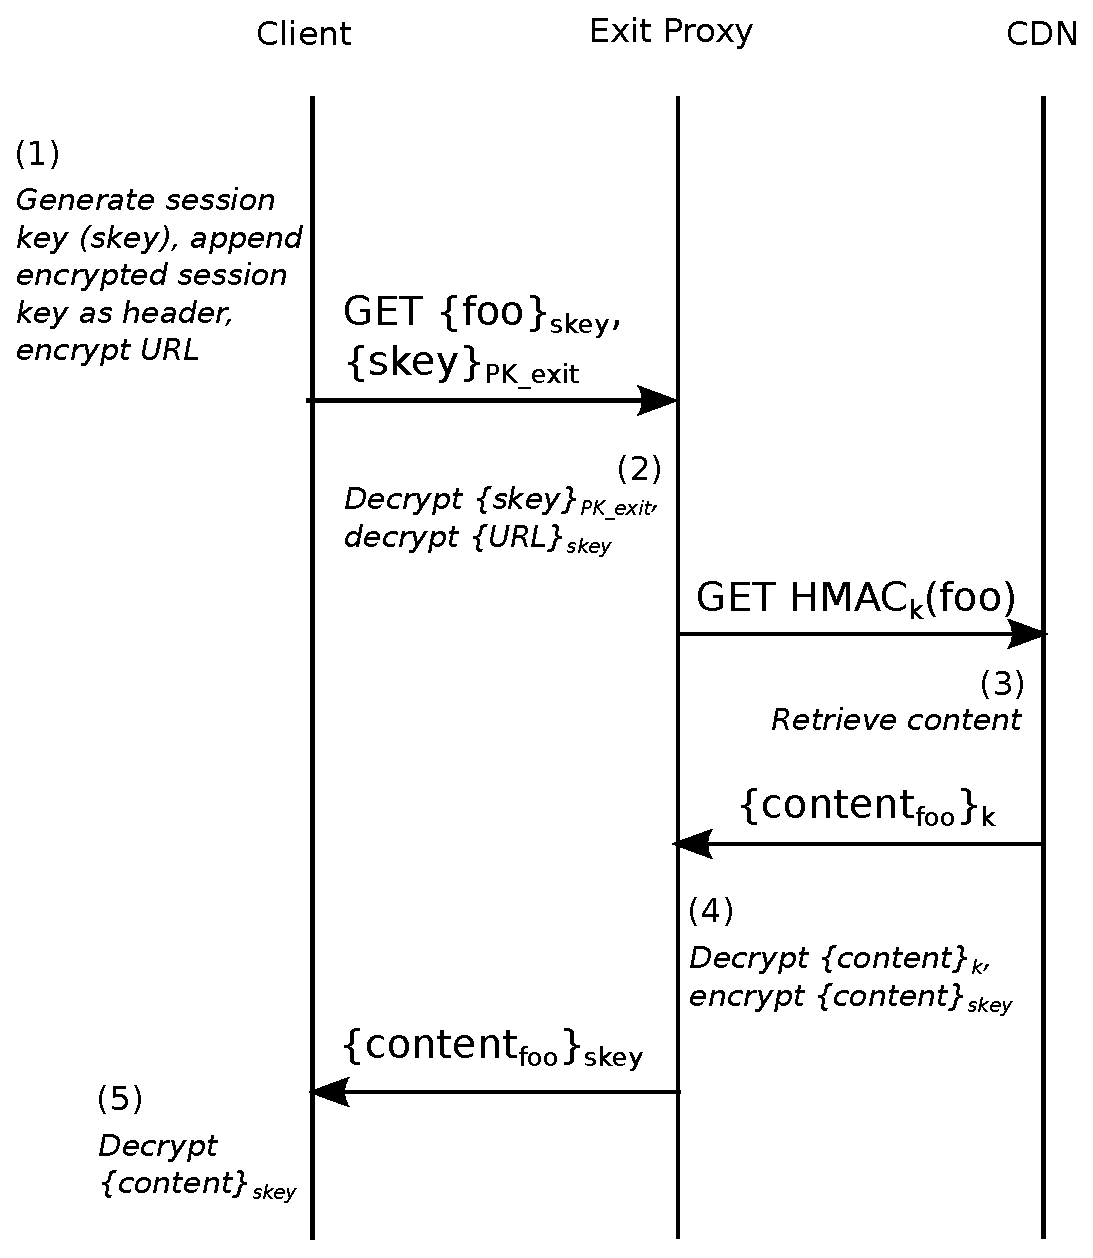
\includegraphics[height=5cm,keepaspectratio]{request_diagram_simple}
%\caption{Steps for retrieving content in \system{} when a client is prioritizing 
%performance and goes directly to an exit proxy.}
%\label{fig:retrieving}
%\end{figure}

\begin{figure}[t!]
\centering
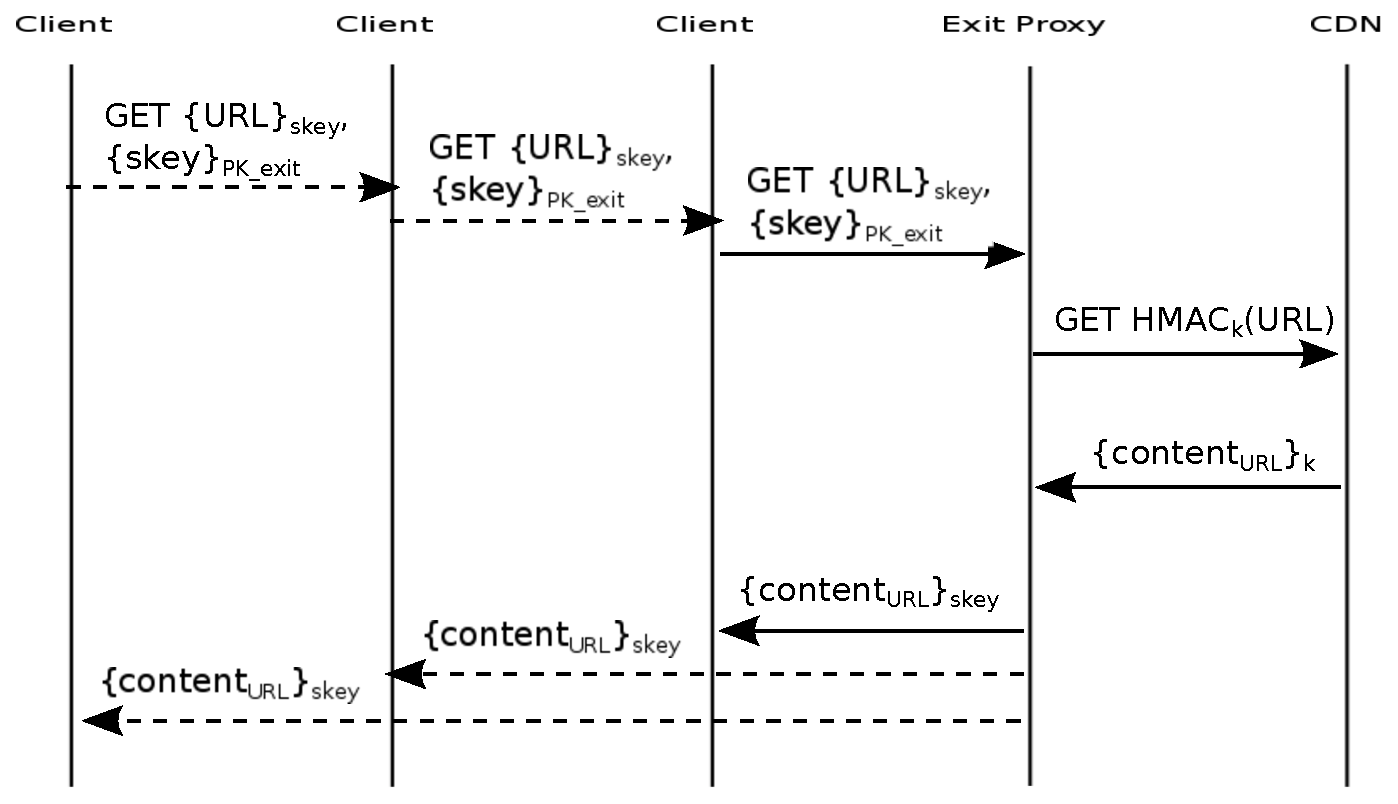
\includegraphics[width=.5\textwidth]{request_diagram_complex}
\caption{Steps for retrieving content in \system{}.  The dotted lines represent 
optional steps for when a client is prioritizing 
privacy and proxies a request through two other clients before reaching the 
exit proxy.  In this case, the request is sent sequentially through peers, 
and the response is sent in a multicast manner back to the clients.}
\label{fig:retrieving2}
\end{figure}

Finally, the exit proxy must send the response back to the correct client without
knowing who the client is.  First, the exit proxy fetches the session key $k_{session}$
that it stored for the corresponding incoming request, and it uses this key to encrypt the response.  Then, it looks up the source route it stored for the corresponding request 
and uses a multicast technique to send to the encrypted response to all clients on the source route.  At this point, the exit proxy can delete the source route and session key entries 
for this request/response.  Only the original (true) client has $k_{session}$, so only the original (true) client can decrypt the response.  All other clients will discard 
the encrypted response because they cannot decrypt it.  

\subsection{Clients Joining \& Leaving}
\label{sec:join}

When a client joins \system{}, it will download \system{} client software.  This
includes information about exit proxy mappings to URLs for which they hold a key, 
software for modifying requests with session keys and source routes, and software 
for running a proxy.  Clients will learn about other clients in the system via 
a gossip protocol.  We do not detail this as gossip protocols have been studied 
extensively in the past~\cite{kermarrec2007gossiping,vogels2003power,eugster2004epidemic}.  
Similarly, when a client leaves the system, this information is propogated to its 
peers using a gossip protocol.  \annie{\system{} scales with increasing numbers of clients and 
exit proxies, which is described in more detail in Section \ref{sec:scalability}.}

\subsection{Partial Deployment}
\label{sec:partial}
\system{} should be partially deployable, in the sense that if only some origin servers participate or only some CDNs participate, then 
the system should still offer some protections.  We outline two different partial
deployment possibilities below.

\textbf{Deployment with Origin Servers' Full Participation.}
One option for deploying \system{} is to ensure there is some set $S$ of origin servers that participate fully in the 
system.  These publishers obfuscate their content, identifiers, and certificates, and most importantly, only have 
obfuscated data stored on the CDNs cache nodes.  $S$ must be greater than one, otherwise the CDN can infer 
that a client accessing this obfuscated content is actually accessing content that can be identified.  This partial deployment plan 
 protects the privacy of the clients accessing the content created by the set of origin servers $S$.  It does not 
protect the clients' privacy as completely as full participation of all origin servers in \system{} because the CDN can 
still view cross site browsing patterns among the origin servers that are not participating. It is important to note though, that 
because the clients are behind proxies, the CDN cannot individually identify users.  The CDN can attribute requests to exit proxies, but 
not to clients.  

\textbf{Deployment with Origin Servers' Partial Participation.} 
Some origin servers may prioritize performance 
and availability.  Therefore, they should have the option to gradually move towards full participation by pushing 
both encrypted and plaintext content to the CDN.  In this partial deployment plan, we see some set of origin servers 
fully participating with only encrypted content, some other set of origin servers partially participating with both 
encrypted and plaintext content, and some last set of publishers that are not participating.  Unfortunately, if 
a publisher has the same content that is both encrypted and plaintext content at a cache node, then an adversary can correlate the access 
patterns on encrypted and plaintext content for the origin server.  In order to prevent this identification of the 
content, \system{} can use encoded URLs (described in Section \ref{sec:design}), which obfuscates the access patterns for 
a given piece of content; this holds true if an origin server chooses to distribute its content in an encrypted manner using \system{}
 and in plaintext form on a different CDN.  In this case, the origin server can still encode its URLs in multiple ways to 
prevent correlating access patterns between the encrypted and plaintext content.  Therefore, this deployment option allows for 
differing levels of participation in the system, while still preserving the protections provided by \system{}.  



%\subsection{Optimizations}
%\label{sec:optimizations}
%While there are some optimizations that CDNs typically perform today that would not be possible with \system{}, the architecture 
%of \system{} allows for new optimizations that are not possible in existing CDNs.  Here we describe how \system{} limits 
%current traditional CDN's optimizations, and then we outline some ways in which \system{} 
%can be optimized in terms of performance.

%CDNs become slightly limited in terms of the possible performance optimizations when following \system{}'s design.  For example, 
%many CDNs perform HTTPS re-writes on content that they cache, but this can only be done if the CDN has access to the 
%decrypted content.  Similarly, the CDN needs the decrypted content to perform minimizations on HTML, CSS, and Javascript 
%files.  While this likely increases performance in traditional CDNs, it does not provide the greatest increase in performance; 
%content caching around the world is the greatest benefit to performance, which \system{} preserves.

%\paragraph{Pre-Fetch DNS Responses} One way to increase the performance of \system{} is to pre-fetch DNS responses at 
%the proxies.  This would allow the proxy to serve each client request faster because it would not have to send 
%as many DNS requests.  Pre-fetching DNS responses would not take up a large amount of space, but it also 
%would not be a complete set of all DNS responses.  Additionally, if the content is moved between cache nodes 
%at the CDN, then DNS response must also change; therefore, the pre-fetched DNS responses should have a 
%lifetime that is shorter than the lifetime of the content on a cache node.

%\paragraph{Load Balance Proxy Selection} As the proxy performs a number of operations on the client's behalf, it 
%runs into the possibility of being overloaded.  \system{} uses consistent hashing to generally address the load balancing 
%problem, but an edge case that may still cause some exit proxies to be overloaded is extremely popular content.  To mitigate this, 
%multiple exit proxies can store the shared key $k$ for the URL that is extremely popular, and therefore divide the load, while 
%still taking advantage of the the CDNs caching benefits.  

%\paragraph{Use \system{} for Partial Content} Different content publishers have different needs, and each content publisher might 
%have different needs for different content.  The design of \system{} allows content publishers to publish some of their content 
%on \system{} and some on other CDNs.  This is useful in a case where some content is more sensitive, while other content needs better 
%performance.  

%\paragraph{Different Modes of Operation}  As briefly mentioned in Section \ref{sec:retrieve}, there are two different modes of 
%operation, where one provides better performance, and the other provides better privacy.  In the first mode, the client 
%can choose to send her request directly to the exit proxy, and not forward her request through any of her peers.  While this 
%allows the exit proxy to identify her, it does not allow the CDN to identify her or her request.  In the second mode, the 
%client forwards her request through a set of peers before it reaches the exit proxy.  In this mode, the client can decide to 
%prepend other clients' identifiers before her own, so it appears as if the request came from a different client.  This 
%provides unlinkability between the client and the request.  This mode also provides the option of {\it only} prepending other clients' 
%identifiers and then forwarding the request directly to the exit proxy; this provides the same performance benefit as the first mode, 
%but also provides unlinkability.  While this seems like the optimal solution, it cannot be the only option because the exit proxy 
%would always know that the true client is the previous hop in the source route.  These two modes of operation provide the client 
%with different ways to use the system both based on their privacy preferences and based on the type of content they are requesting.
